\documentclass[11pt,a4paper]{article}

% --- Essential Packages ---
\usepackage[utf8]{inputenc}
\usepackage[T1]{fontenc}
\usepackage{amsmath,amssymb,amsfonts}
\usepackage{graphicx}
\usepackage{booktabs}
\usepackage{geometry}
\usepackage{hyperref}
\usepackage{xcolor}
\usepackage{fancyhdr}
\usepackage{subcaption}
\usepackage{float}
\usepackage{microtype}

% --- Page Margins ---
\geometry{
    top=2.5cm,
    bottom=2.5cm,
    left=2.5cm,
    right=2.5cm
}

% --- Hyperref Setup ---
\hypersetup{
    colorlinks=true,
    linkcolor=blue!70!black,
    citecolor=blue!70!black,
    urlcolor=blue!80!black
}

% --- Header and Footer ---
\pagestyle{fancy}
\fancyhf{}
\rhead{\small \textit{Mechanics Applied to Aerospace Engineering --- Lab 1}}
\lhead{\small \textit{UC3M --- Aerospace Engineering}}
\cfoot{\thepage}

% --- Document Metadata ---
\title{\vspace{-1.5cm}
    \textbf{\Large Laboratory Session 1: Particle Connected to a Spool} \\
    \large Kinematic Modeling, Numerical Integration, and Event Analysis
}

\author{
    \textbf{Group LA} \\[0.5em]
    \small Ismael Mart\'in D\'iez \quad (NIA: 100XXXXXX) \\
    \small David Mart\'in Garc\'ia \quad (NIA: 100XXXXXX) \\
    \small Alejandro Ranz Remart\'inez \quad (NIA: 100XXXXXX) \\[0.5em]
    \small \textit{Bachelor in Aerospace Engineering} \\
    \small \textit{Department of Bioengineering and Aerospace Engineering, Universidad Carlos III de Madrid} \\
    \small Course: \textit{Mechanics Applied to Aerospace Engineering (251-14165)}
}
\date{Academic Year 2026--2027}

\begin{document}

\maketitle

\begin{abstract}
This report presents the analytical formulation and numerical simulation of the planar motion of a heavy particle suspended by an inextensible string wrapped around a rotating cylinder of radius $a$. Using a polar coordinate system attached to the moving point of tangency, the equations of motion are projected onto the direction perpendicular to the cable, decoupling the angular acceleration $\ddot{\phi}$ from the unknown string tension. This reduces the problem to a single second-order nonlinear differential equation for the tangency angle $\phi(t)$. Numerical integration is carried out in MATLAB using \texttt{ode45} with an event-detection function (\texttt{stopfun}) that halts execution when the particle strikes the cylinder ($\xi \le 0$) or when the string loses tension ($T \le 0$). Five study cases are investigated to evaluate mechanical energy conservation for a fixed cylinder ($\omega = 0$), non-conservative work done by cylinder rotation ($\omega \neq 0$), the physical singularity during spool impact in Case 3, and the transition to 2-DoF ballistic flight upon string slackening in Case 4.
\end{abstract}

---

\section{Introduction}

In this laboratory session, we analyze the planar dynamics of a point-mass particle suspended by a thin, flexible, inextensible string that winds or unwinds around a cylindrical spool rotating at a constant angular speed $\omega$. The unspooled segment of the string continuously changes length as the contact point between the string and the cylinder moves along the circumference. 

The main objectives of this work are:
\begin{enumerate}
    \item Derive the kinematic vectors (position, velocity, and acceleration) and the equations of motion from Newton's Second Law.
    \item Determine the configuration degrees of freedom and obtain closed-form expressions for the angular acceleration $\ddot{\phi}$ and string tension $T(t)$.
    \item Implement a standalone MATLAB script using \texttt{ode45} and event handling (\texttt{stopfun}) to numerically simulate the motion and detect physical stopping conditions.
    \item Analyze the five study cases defined in the laboratory guidelines, verifying energy conservation, explaining why simulations terminate, and detailing the code modifications required when the string becomes slack.
\end{enumerate}

The report is organized following the 11 items outlined in the laboratory session guidelines.

---

\section{Analytical Formulation (Items 1--4, 9)}
\label{sec:methodology}

\subsection{Item 1: Degrees of Freedom and Kinematic Constraint}
We consider a rigid cylinder of radius $a$ centered at the origin $O$ of an inertial Cartesian reference frame $(O; x, y)$ with gravity acting in the $-\hat{j}$ direction. The cylinder rotates counterclockwise at a constant angular rate $\vec{\omega} = \omega\hat{k}$. A thin, massless, inextensible string of total length $l$ leaves the spool tangentially at point $B$. The radial vector $\vec{r}_O^B$ forms an angle $\phi(t)$ with the horizontal axis $Ox$.

Let $s_{\text{wrap}}(t)$ be the length of string wrapped around the cylinder from a fixed attachment point on the spool $A(t)$ to the separation point $B(t)$. Because the cylinder rotates at rate $\omega$, the angular position of the attachment point is $\theta_A(t) = \theta_A(0) + \omega t$. The wrapped length is:
\begin{equation}
    s_{\text{wrap}}(t) = a\left(\omega t - \phi(t)\right) + s_0.
\end{equation}
Since the total string length is constant ($l = s_{\text{wrap}}(t) + \xi(t) = \text{const}$), the unspooled straight length $\xi(t)$ is constrained by:
\begin{equation}
    \label{eq:constraint_xi}
    \xi(t) = \xi_0 - a\left(\omega t - \phi(t)\right) = \xi_0 + a\left(\phi(t) - \omega t\right),
\end{equation}
where $\xi_0 = \xi(0) = 1\text{ m}$ is the initial unspooled length at $t = 0$ when $\phi(0) = 0$. Differentiating Eq. \eqref{eq:constraint_xi} with respect to time yields:
\begin{equation}
    \label{eq:xi_dot}
    \dot{\xi}(t) = a\dot{\phi}(t) - a\omega.
\end{equation}

\noindent\textbf{Configuration Degrees of Freedom (C.D.O.F.):} In the plane, the particle position is defined by two generalized coordinates $(\xi, \phi)$. Since Eq. \eqref{eq:constraint_xi} provides one holonomic constraint equation relating $\xi$ and $\phi$:
\begin{equation}
    \text{C.D.O.F.} = 2 - 1 = 1.
\end{equation}
The system has **1 configuration degree of freedom**, parameterized by $\phi(t)$. When $\omega \neq 0$, the constraint depends explicitly on time, making the system **rheonomic**. When $\omega = 0$, the constraint is time-independent, making the system **scleronomic**.

\subsection{Item 2: Kinematic Vectors of Particle $P$}
We define a moving polar basis attached to the radius vector $OB$:
\begin{align}
    \label{eq:basis_er}
    \hat{e}_r &= \cos\phi\,\hat{i} + \sin\phi\,\hat{j}, \\
    \label{eq:basis_ephi}
    \hat{e}_\phi &= -\sin\phi\,\hat{i} + \cos\phi\,\hat{j}.
\end{align}
Their time derivatives follow Poisson's relation:
\begin{equation}
    \label{eq:basis_derivs}
    \dot{\hat{e}}_r = \dot{\phi}\,\hat{e}_\phi, \qquad \dot{\hat{e}}_\phi = -\dot{\phi}\,\hat{e}_r.
\end{equation}
In terms of this basis, the Cartesian unit vectors are:
\begin{equation}
    \label{eq:cartesian_in_polar}
    \hat{i} = \hat{e}_r\cos\phi - \hat{e}_\phi\sin\phi, \qquad \hat{j} = \hat{e}_r\sin\phi + \hat{e}_\phi\cos\phi.
\end{equation}

\subsubsection{Position Vector $\vec{r}_P$}
The position of tangency point $B$ is $\vec{r}_B = a\hat{e}_r$. The straight string segment of length $\xi$ extends perpendicularly along $-\hat{e}_\phi$:
\begin{equation}
    \label{eq:pos_vector}
    \vec{r}_P(t) = a\hat{e}_r - \xi(t)\hat{e}_\phi.
\end{equation}
In Cartesian coordinates:
\begin{equation}
    \label{eq:pos_cartesian}
    x_P(t) = a\cos\phi + \xi\sin\phi, \qquad y_P(t) = a\sin\phi - \xi\cos\phi.
\end{equation}

\subsubsection{Velocity Vector $\vec{v}_P$}
Differentiating Eq. \eqref{eq:pos_vector} with respect to time:
\begin{equation}
    \vec{v}_P = \frac{d\vec{r}_P}{dt} = a\dot{\hat{e}}_r - \dot{\xi}\hat{e}_\phi - \xi\dot{\hat{e}}_\phi = a\dot{\phi}\hat{e}_\phi - \dot{\xi}\hat{e}_\phi + \xi\dot{\phi}\hat{e}_r.
\end{equation}
Substituting $\dot{\xi} = a\dot{\phi} - a\omega$ from Eq. \eqref{eq:xi_dot}:
\begin{equation}
    \vec{v}_P = a\dot{\phi}\hat{e}_\phi - (a\dot{\phi} - a\omega)\hat{e}_\phi + \xi\dot{\phi}\hat{e}_r.
\end{equation}
The terms $a\dot{\phi}\hat{e}_\phi$ cancel, leaving:
\begin{equation}
    \label{eq:vel_vector}
    \vec{v}_P(t) = \xi\dot{\phi}\,\hat{e}_r + a\omega\,\hat{e}_\phi.
\end{equation}
In Cartesian components:
\begin{equation}
    \label{eq:vel_cartesian}
    \dot{x}_P(t) = -a\omega\sin\phi + \xi\dot{\phi}\cos\phi, \qquad \dot{y}_P(t) = a\omega\cos\phi + \xi\dot{\phi}\sin\phi.
\end{equation}
When the spool is stationary ($\omega = 0$), the component along the string is zero ($\vec{v}_P \cdot \hat{e}_\phi = 0$), so the particle moves purely perpendicular to the straight string segment. When $\omega \neq 0$, the particle also receives an axial feed velocity $a\omega$ along $\hat{e}_\phi$.

\subsubsection{Acceleration Vector $\vec{a}_P$}
Differentiating Eq. \eqref{eq:vel_vector} with respect to time:
\begin{align}
    \vec{a}_P &= \frac{d\vec{v}_P}{dt} = (\dot{\xi}\dot{\phi} + \xi\ddot{\phi})\hat{e}_r + \xi\dot{\phi}\dot{\hat{e}}_r + a\omega\dot{\hat{e}}_\phi \nonumber \\
    &= (\dot{\xi}\dot{\phi} + \xi\ddot{\phi})\hat{e}_r + \xi\dot{\phi}^2\hat{e}_\phi - a\omega\dot{\phi}\hat{e}_r.
\end{align}
Substituting $\dot{\xi} = a\dot{\phi} - a\omega$:
\begin{equation}
    \vec{a}_P = \left[(a\dot{\phi} - a\omega)\dot{\phi} + \xi\ddot{\phi} - a\omega\dot{\phi}\right]\hat{e}_r + \xi\dot{\phi}^2\hat{e}_\phi.
\end{equation}
Simplifying:
\begin{equation}
    \label{eq:acc_vector}
    \vec{a}_P(t) = \left(a\dot{\phi}^2 + \xi\ddot{\phi} - 2a\omega\dot{\phi}\right)\hat{e}_r + \xi\dot{\phi}^2\hat{e}_\phi.
\end{equation}

\subsection{Item 3: Forces Acting on Particle $P$}
The forces acting on the particle are:
\begin{enumerate}
    \item \textbf{String Tension $\vec{T}$:} Acts along the string segment towards point $B$ ($+\hat{e}_\phi$ direction):
    \begin{equation}
        \label{eq:force_T}
        \vec{T} = T\,\hat{e}_\phi, \qquad (T \ge 0).
    \end{equation}
    \item \textbf{Gravity $\vec{F}_g$:} Acts vertically downwards ($-\hat{j}$). Using Eq. \eqref{eq:cartesian_in_polar}:
    \begin{equation}
        \label{eq:force_g}
        \vec{F}_g = -mg\hat{j} = -mg\left(\sin\phi\,\hat{e}_r + \cos\phi\,\hat{e}_\phi\right).
    \end{equation}
\end{enumerate}

\subsection{Item 4: Equations of Motion and String Tension}
Applying Newton's Second Law ($\sum \vec{F} = m\vec{a}_P$):
\begin{equation}
    -mg\sin\phi\,\hat{e}_r + (T - mg\cos\phi)\,\hat{e}_\phi = m\left(a\dot{\phi}^2 + \xi\ddot{\phi} - 2a\omega\dot{\phi}\right)\hat{e}_r + m\xi\dot{\phi}^2\hat{e}_\phi.
\end{equation}

\subsubsection{Radial Component ($\hat{e}_r$): Decoupled ODE for $\ddot{\phi}$}
Projecting onto the radial unit vector $\hat{e}_r$ eliminates tension $T$ since $\vec{T} \cdot \hat{e}_r = 0$:
\begin{equation}
    m\left(a\dot{\phi}^2 + \xi\ddot{\phi} - 2a\omega\dot{\phi}\right) = -mg\sin\phi.
\end{equation}
Dividing by $m$ and solving for $\ddot{\phi}$:
\begin{equation}
    \label{eq:ode_phi_final}
    \ddot{\phi}(t) = \frac{-g\sin\phi - a\dot{\phi}^2 + 2a\omega\dot{\phi}}{\xi_0 - a(\omega t - \phi)}.
\end{equation}
This is the second-order nonlinear differential equation governing the motion of the particle.

\subsubsection{Tangential Component ($\hat{e}_\phi$): String Tension $T(t)$}
Projecting onto $\hat{e}_\phi$:
\begin{equation}
    T - mg\cos\phi = m\xi\dot{\phi}^2.
\end{equation}
Solving for $T$:
\begin{equation}
    \label{eq:tension_final}
    T(t, \phi, \dot{\phi}) = m\xi\dot{\phi}^2 + mg\cos\phi.
\end{equation}

\subsection{Item 9: Mechanical Energy and Conservation}
The total mechanical energy $E(t) = E_k + E_p$ taking the datum at $y = 0$ is:
\begin{equation}
    \label{eq:energy_final}
    E(t) = \frac{1}{2}m\|\vec{v}_P\|^2 + mgy_P = \frac{1}{2}m\left(\xi^2\dot{\phi}^2 + a^2\omega^2\right) + mg\left(a\sin\phi - \xi\cos\phi\right).
\end{equation}
The power delivered by the non-conservative string tension force is:
\begin{equation}
    P_T = \vec{T} \cdot \vec{v}_P = \left(T\hat{e}_\phi\right) \cdot \left(\xi\dot{\phi}\hat{e}_r + a\omega\hat{e}_\phi\right) = a\omega\,T(t).
\end{equation}
Therefore, the rate of change of mechanical energy is:
\begin{equation}
    \label{eq:dE_dt}
    \frac{dE}{dt} = a\omega\,T(t).
\end{equation}
\begin{itemize}
    \item When $\omega = 0$ (stationary cylinder): $dE/dt = 0$, so **mechanical energy is strictly conserved**.
    \item When $\omega \neq 0$ (rotating cylinder): $dE/dt = a\omega T > 0$, so the rotating spool does positive work on the particle, increasing its mechanical energy over time.
\end{itemize}

---

\section{Numerical Implementation (Items 5 \& 6)}
\label{sec:numerical}

\subsection{Item 5: State-Space Formulation for \texttt{ode45}}
To integrate Eq. \eqref{eq:ode_phi_final} with MATLAB's \texttt{ode45}, we define the state vector $\mathbf{X} = [X_1; X_2] = [\phi; \dot{\phi}]$:
\begin{equation}
    \label{eq:state_space}
    \frac{d\mathbf{X}}{dt} = \begin{bmatrix} \dot{X}_1 \\ \dot{X}_2 \end{bmatrix} = \begin{bmatrix} X_2 \\ \dfrac{-g\sin X_1 - aX_2^2 + 2a\omega X_2}{\xi_0 - a(\omega t - X_1)} \end{bmatrix}.
\end{equation}

\noindent\textbf{Initial Velocity Conversion:} At $t = 0$, $\phi(0) = 0$ and $\xi(0) = \xi_0 = 1.0\text{ m}$. From Eq. \eqref{eq:vel_cartesian}:
\begin{equation}
    v_{x0} = \dot{x}_P(0) = \xi_0\dot{\phi}(0) \implies \dot{\phi}(0) = \frac{v_{x0}}{\xi_0}.
\end{equation}
Since $\xi_0 = 1.0\text{ m}$, $\dot{\phi}(0) = v_{x0}$ numerically.

\subsection{Item 6: Event Handling Function (\texttt{stopfun})}
The physical simulation must terminate when either of the following events occurs:
\begin{enumerate}
    \item The particle reaches the surface of the cylinder: $\xi(t) \le 0$.
    \item The string becomes slack: $T(t) \le 0$.
\end{enumerate}
As $\xi \to 0$, the denominator in Eq. \eqref{eq:state_space} approaches zero, producing an algebraic singularity ($\ddot{\phi} \to \infty$). To prevent \texttt{ode45} from stalling with infinitesimal step sizes, physical contact is defined when $\xi(t)$ reaches a small clearance $\epsilon_{\text{contact}} = 10^{-3}\text{ m}$ (1 mm):
\begin{equation}
    \mathbf{value} = \begin{bmatrix} \xi(t) - \epsilon_{\text{contact}} \\ T(t) \end{bmatrix}, \qquad \mathbf{isterminal} = \begin{bmatrix} 1 \\ 1 \end{bmatrix}, \qquad \mathbf{direction} = \begin{bmatrix} -1 \\ -1 \end{bmatrix}.
\end{equation}
Setting $\mathbf{direction} = [-1; -1]$ triggers the event only when crossing the zero boundary from positive to negative.

---

\section{Results and Simulation Analysis (Items 7, 8, 10, 11)}
\label{sec:results}

The model was integrated using the lab parameters: $g = 9.81\text{ m/s}^2$, $m = 0.1\text{ kg}$, $a = 0.20\text{ m}$, $\xi_0 = 1.0\text{ m}$, and $\phi(0) = 0\text{ rad}$. The results for the five study cases are summarized in Table \ref{tab:cases_summary}.

\begin{table}[H]
    \centering
    \caption{Simulation summary across all five study cases.}
    \label{tab:cases_summary}
    \begin{tabular}{ccccccc}
        \toprule
        \textbf{Case} & $\boldsymbol{\omega}$ [rad/s] & $\boldsymbol{v_{x0}}$ [m/s] & $\boldsymbol{\dot{\phi}(0)}$ [rad/s] & $\boldsymbol{E_0}$ [J] & $\boldsymbol{t_{\text{stop}}}$ [s] & \textbf{Termination Reason} \\
        \midrule
        \textbf{Case 1} & $0.1$ & $0.0$   & $0.0$   & $-0.9790$ & $49.9500$ & Hits spool surface ($\xi \to 0$) \\
        \textbf{Case 2} & $0.0$ & $-1.0$  & $-1.0$  & $-0.9310$ & $20.0000$ & Max time reached (periodic oscillation) \\
        \textbf{Case 3} & $0.0$ & $-10.0$ & $-10.0$ & $4.0210$  & $0.2709$  & Hits spool surface ($\xi \to 0$) \\
        \textbf{Case 4} & $0.0$ & $+4.0$  & $+4.0$  & $-0.1810$ & $1.6935$  & String slackens ($T = 0$ at $\phi = -1.59\text{ rad}$) \\
        \textbf{Case 5} & $0.1$ & $+1.0$  & $+1.0$  & $-0.9290$ & $35.5094$ & Hits spool surface ($\xi \to 0$) \\
        \bottomrule
    \end{tabular}
\end{table}

\begin{figure}[H]
    \centering
    \begin{subfigure}[b]{0.48\textwidth}
        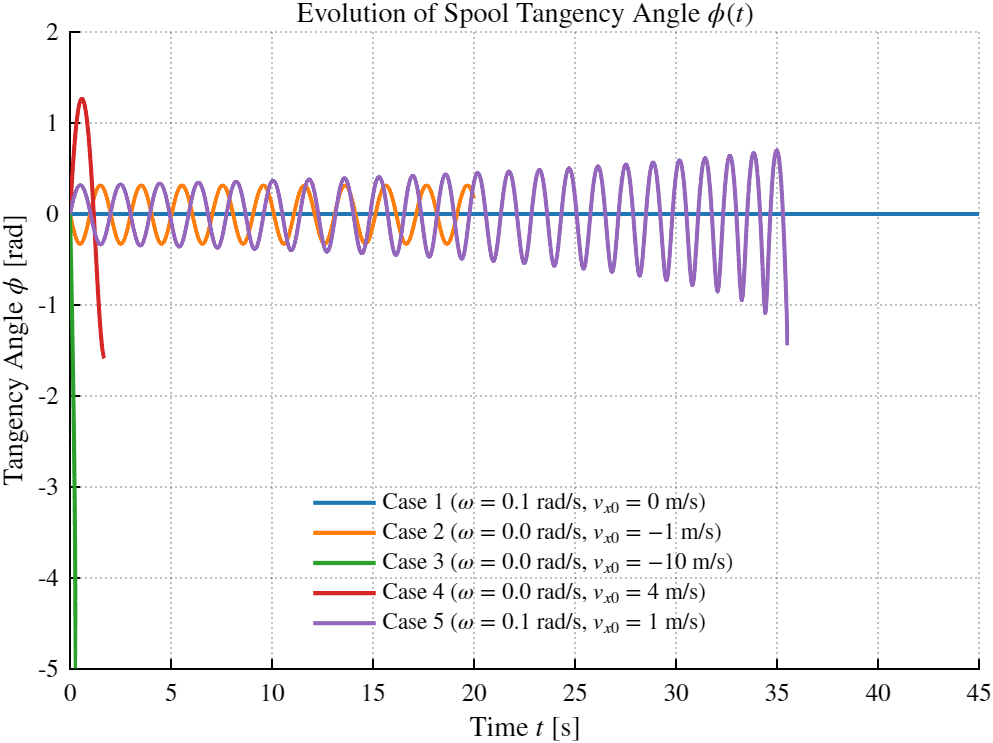
\includegraphics[width=\textwidth]{figs/fig1_phi_evolution.png}
        \caption{Tangency angle $\phi(t)$.}
        \label{fig:phi_evol}
    \end{subfigure}
    \hfill
    \begin{subfigure}[b]{0.48\textwidth}
        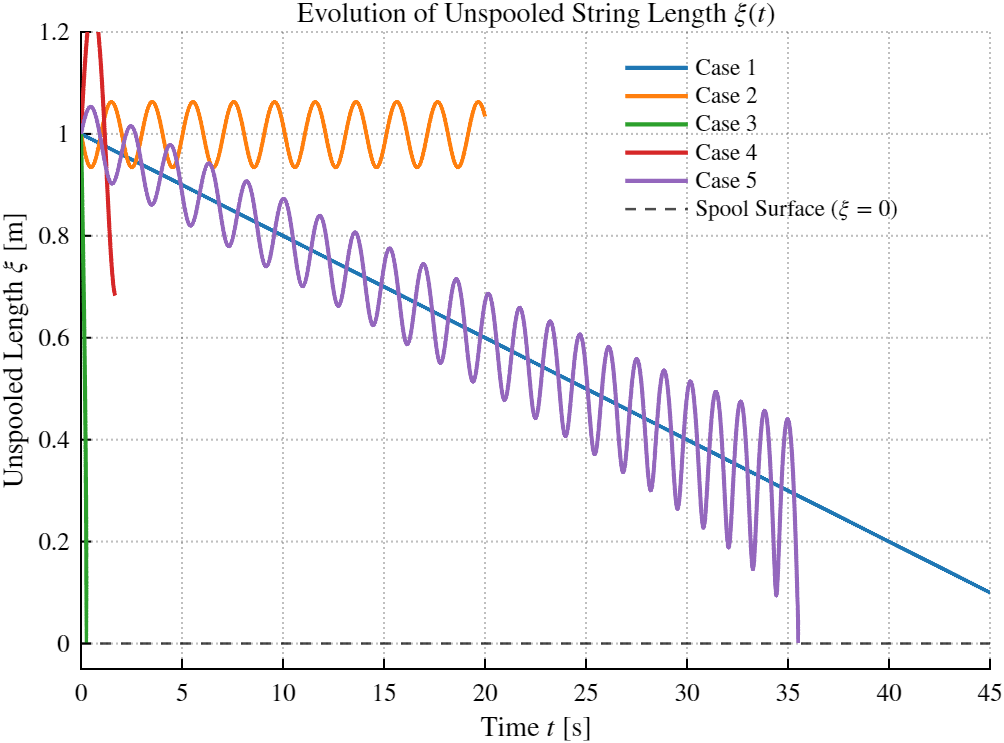
\includegraphics[width=\textwidth]{figs/fig2_xi_evolution.png}
        \caption{Unspooled string length $\xi(t)$.}
        \label{fig:xi_evol}
    \end{subfigure}
    \caption{Time histories of coordinates $\phi(t)$ and unspooled length $\xi(t)$.}
    \label{fig:state_variables}
\end{figure}

\begin{figure}[H]
    \centering
    \begin{subfigure}[b]{0.48\textwidth}
        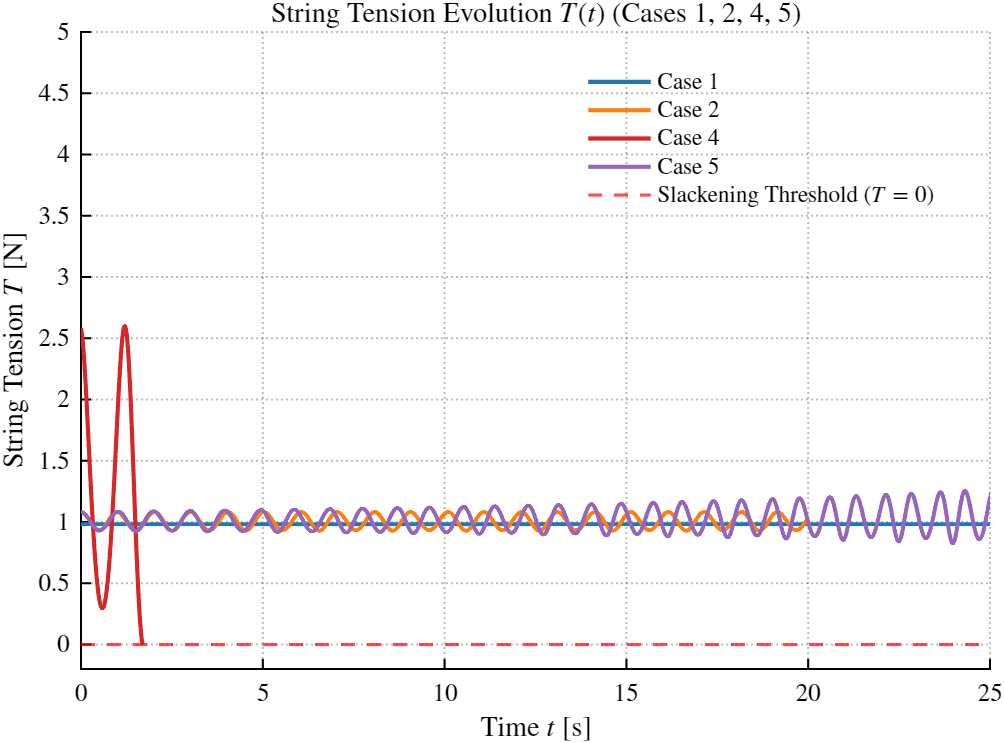
\includegraphics[width=\textwidth]{figs/fig3_tension_evolution.png}
        \caption{String tension $T(t)$ (Cases 1, 2, 4, 5).}
        \label{fig:tension_evol}
    \end{subfigure}
    \hfill
    \begin{subfigure}[b]{0.48\textwidth}
        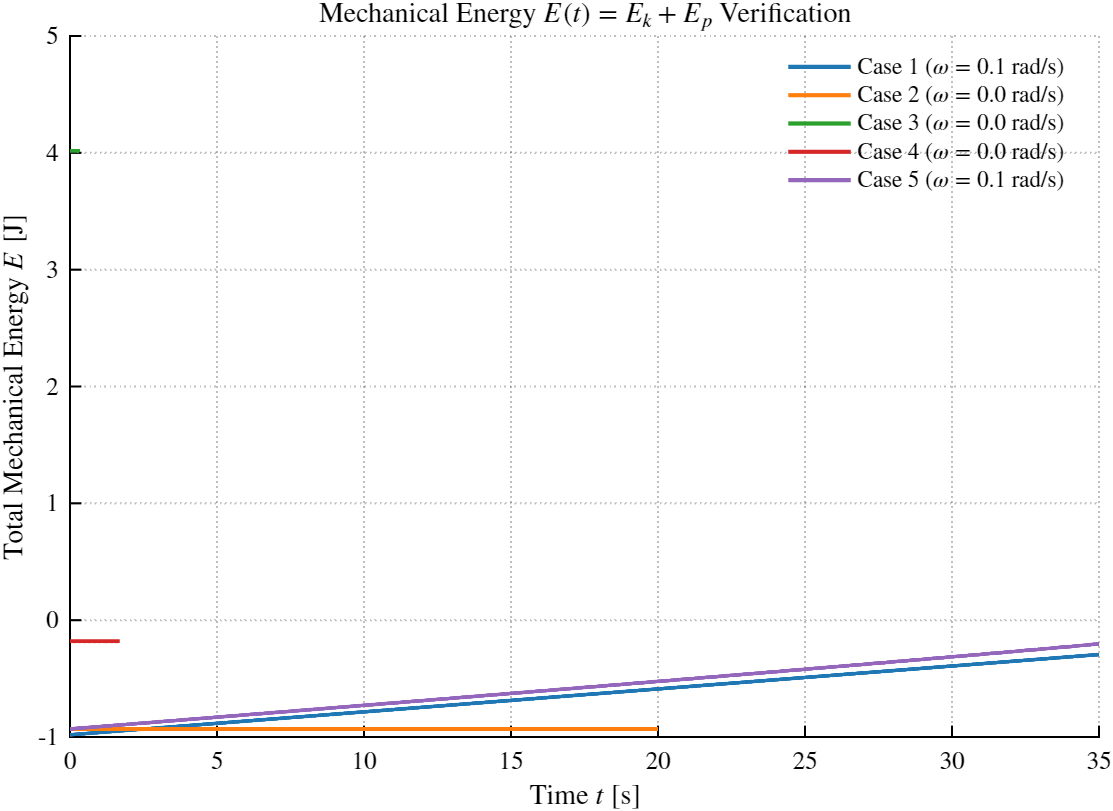
\includegraphics[width=\textwidth]{figs/fig5_mechanical_energy.png}
        \caption{Total mechanical energy $E(t)$.}
        \label{fig:energy_evol}
    \end{subfigure}
    \caption{String tension history and mechanical energy verification.}
    \label{fig:dynamics_energy}
\end{figure}

\begin{figure}[H]
    \centering
    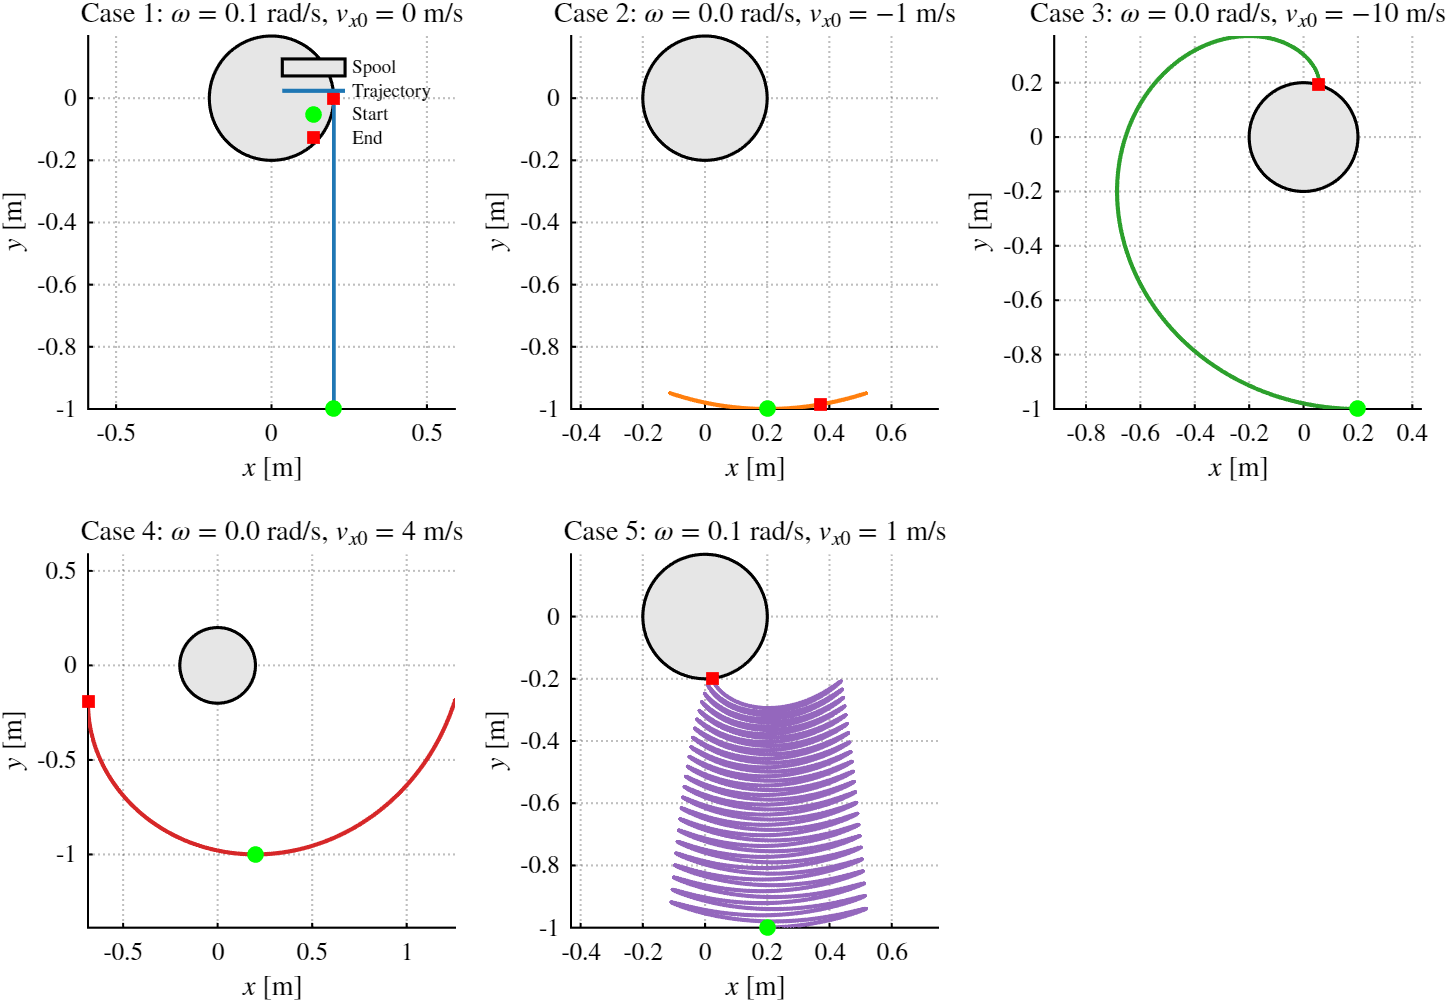
\includegraphics[width=0.88\textwidth]{figs/fig4_trajectories_Oxy.png}
    \caption{Trajectories of particle $P$ in Cartesian coordinates $Oxy$ for all five cases. The spool cylinder ($a = 0.20\text{ m}$) is shown in gray, initial positions are green circles, and final states are red squares.}
    \label{fig:trajectories}
\end{figure}

\subsection{Detailed Case-by-Case Discussion (Item 10)}
\begin{itemize}
    \item \textbf{Case 1 ($\omega = 0.1\text{ rad/s}, v_{x0} = 0\text{ m/s}$):} With zero initial velocity, gravity and tension remain vertical along $x = a = 0.20\text{ m}$. The particle does not swing ($\phi(t) \equiv 0$). The spool reels in the string at speed $v_{\text{reel}} = a\omega = 0.02\text{ m/s}$. The particle ascends vertically and reaches the cylinder at $t = \xi_0 / (a\omega) = 50.00\text{ s}$ (detected at $49.95\text{ s}$ by the $1\text{ mm}$ clearance). The tension is constant at $T = mg = 0.981\text{ N}$, and the cylinder does work at power $P = a\omega mg = 0.01962\text{ W}$, causing a linear increase in energy (Fig. \ref{fig:energy_evol}).
    \item \textbf{Case 2 ($\omega = 0\text{ rad/s}, v_{x0} = -1.0\text{ m/s}$):} The spool is stationary and the initial velocity is moderate. The particle executes stable periodic oscillations around $\phi = 0$. String tension remains positive throughout ($0.8\text{ N} \le T \le 1.2\text{ N}$), avoiding slackening. Because $\omega = 0$, mechanical energy is strictly conserved at $E = -0.9310\text{ J}$. The simulation runs to the maximum time $t = 20\text{ s}$.
    \item \textbf{Case 3 ($\omega = 0\text{ rad/s}, v_{x0} = -10.0\text{ m/s}$):} Due to the high initial velocity, the particle rapidly winds around the cylinder, spiraling inward and striking the surface at $t = 0.2709\text{ s}$ at $\phi = -5.00\text{ rad}$ ($-286.5^\circ$). Energy is conserved at $E = 4.0210\text{ J}$ until impact.
    \item \textbf{Case 4 ($\omega = 0\text{ rad/s}, v_{x0} = 4.0\text{ m/s}$):} The particle swings upwards to the left. As potential energy increases, its velocity decreases. At $t = 1.6935\text{ s}$ and $\phi = -1.5859\text{ rad}$, the centripetal reaction $m\xi\dot{\phi}^2$ is no longer large enough to balance the inward component of gravity $-mg\cos\phi$. String tension vanishes ($T = 0$), causing the string to become slack.
    \item \textbf{Case 5 ($\omega = 0.1\text{ rad/s}, v_{x0} = 1.0\text{ m/s}$):} Combines an initial swing with continuous winding by the spool. As the string shortens, the oscillation frequency increases until the particle strikes the cylinder at $t = 35.5094\text{ s}$ ($\phi = -1.444\text{ rad}$). The termination is caused by spool collision ($\xi \to 0$).
\end{itemize}

\subsection{Physical Explanation of Critical Events (Item 10)}

\subsubsection{Singularity at Spool Impact (Case 3)}
As $\xi \to 0$, the denominator in Eq. \eqref{eq:ode_phi_final} approaches zero. Physically, for $\omega = 0$, energy conservation requires:
\begin{equation}
    E_0 = \frac{1}{2}m\xi^2\dot{\phi}^2 + mgy_P = \text{const}.
\end{equation}
Since potential energy $mgy_P$ remains bounded between $\pm mga$, the kinetic term $\frac{1}{2}m(\xi\dot{\phi})^2$ must remain finite. Consequently, as $\xi \to 0$, the angular speed must diverge:
\begin{equation}
    |\dot{\phi}(t)| \sim \frac{\sqrt{2(E_0 - mgy_P)/m}}{\xi(t)} \xrightarrow[\xi \to 0]{} \infty.
\end{equation}
Figure \ref{fig:case3_sing} illustrates this behavior: $|\dot{\phi}|$ surges from $10\text{ rad/s}$ to over $8750\text{ rad/s}$ in the final millisecond. This divergence reflects the conservation of angular momentum about the instantaneous tangency point as the moment of inertia $I = m\xi^2$ vanishes.

\begin{figure}[H]
    \centering
    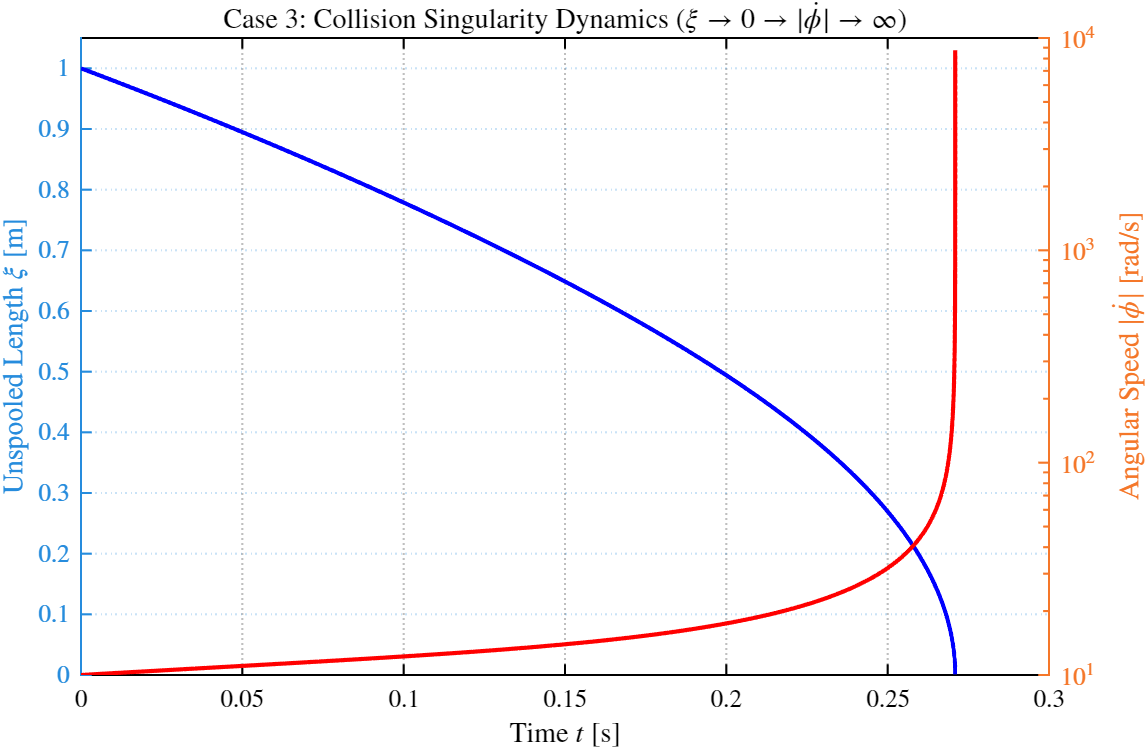
\includegraphics[width=0.68\textwidth]{figs/fig7_case3_singularity.png}
    \caption{Case 3 singularity: rapid collapse of string length $\xi \to 0$ and divergence of angular speed $|\dot{\phi}|$ plotted on a logarithmic scale.}
    \label{fig:case3_sing}
\end{figure}

\subsection{Modifications Required When String Becomes Slack (Item 11)}
When string tension reaches zero ($T = 0$), an inextensible string cannot sustain compressive stress and buckles. The 1-DoF constrained model is no longer physically valid.

To simulate the motion beyond the slackening point $t_{\text{slack}} = 1.6935\text{ s}$, the code must be modified as follows:
\begin{enumerate}
    \item \textbf{Transition Detection:} The event function detects $T \le 0$ and stops the 1-DoF integration at $t_{\text{slack}}$.
    \item \textbf{Switch to 2-DoF Ballistic Flight:} Once the string is slack ($T = 0$), the particle moves solely under gravity ($\vec{F} = -mg\hat{j}$). The governing equations in Cartesian coordinates become:
    \begin{equation}
        \ddot{x}_P = 0, \qquad \ddot{y}_P = -g.
    \end{equation}
    \item \textbf{Initial Conditions for Ballistic Phase:} The initial position and velocity for the ballistic trajectory are set equal to the state of the particle at the moment of slackening:
    \begin{equation}
        \vec{r}_P(t_{\text{slack}}) = \begin{bmatrix} -0.680 \\ -0.198 \end{bmatrix}\text{ m}, \qquad \vec{v}_P(t_{\text{slack}}) = \begin{bmatrix} 0.012 \\ -0.466 \end{bmatrix}\text{ m/s}.
    \end{equation}
    The resulting trajectory is a standard parabola:
    \begin{equation}
        x_P(t) = x(t_{\text{slack}}) + \dot{x}(t_{\text{slack}})\tau, \qquad y_P(t) = y(t_{\text{slack}}) + \dot{y}(t_{\text{slack}})\tau - \frac{1}{2}g\tau^2,
    \end{equation}
    where $\tau = t - t_{\text{slack}}$.
    \item \textbf{Subsequent Event Detection:} During ballistic flight, a new event function must monitor the distance from the particle to the spool tangency point:
    \begin{equation}
        d(t) = \|\vec{r}_P(t) - \vec{r}_B(t)\|.
    \end{equation}
    When $d(t) = \xi(t_{\text{slack}})$, the string straightens and becomes taut again, at which point the model returns to constrained motion. If $\|\vec{r}_P(t)\| \le a$, the particle impacts the spool surface.
\end{enumerate}

Figure \ref{fig:case4_ball} illustrates this ballistic extension implemented in MATLAB, showing the continuous transition from the constrained swinging phase to parabolic free fall.

\begin{figure}[H]
    \centering
    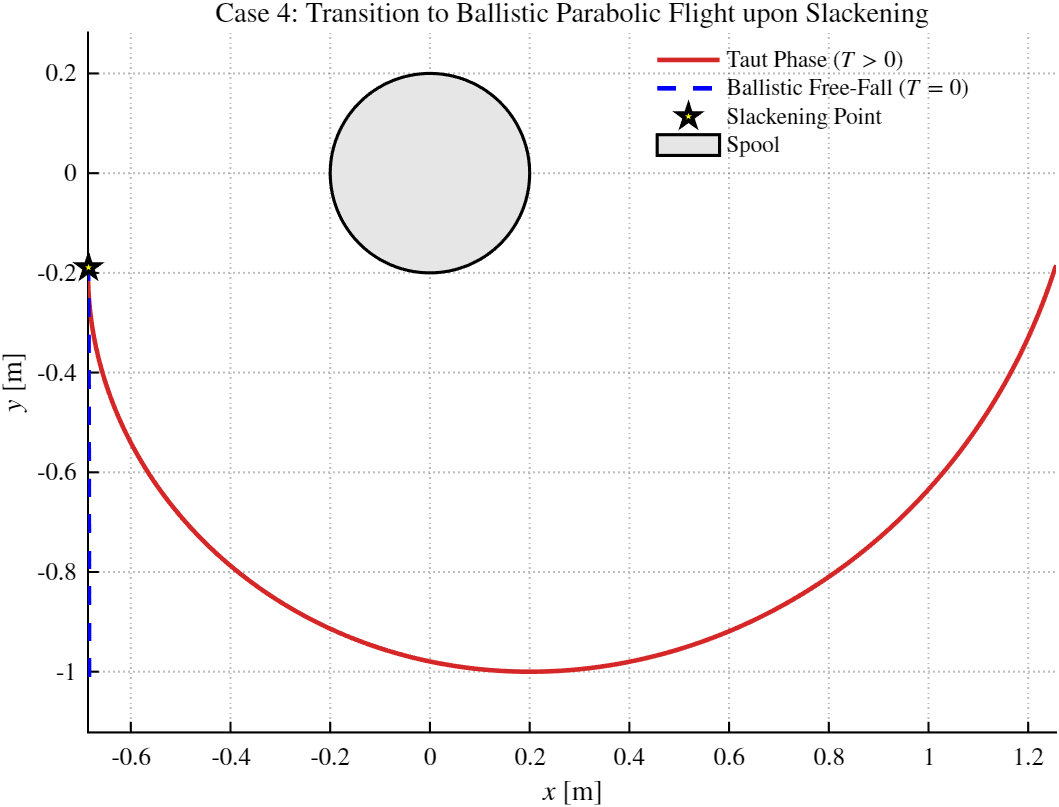
\includegraphics[width=0.68\textwidth]{figs/fig6_case4_ballistic.png}
    \caption{Case 4 trajectory continuation: Stage 1 represents the taut string phase ($T > 0$), and Stage 2 shows the unconstrained ballistic parabolic free fall after tension is lost at $T = 0$.}
    \label{fig:case4_ball}
\end{figure}

---

\section{Conclusions}
\label{sec:conclusions}

In this laboratory work, the dynamics of a point-mass particle connected to a rotating spool was analyzed analytically and integrated numerically in MATLAB:
\begin{enumerate}
    \item \textbf{Kinematic & Dynamic Formulation:} Projecting Newton's Second Law onto the radial direction $\hat{e}_r$ eliminated string tension, producing a single second-order nonlinear ODE governing the single degree of freedom $\phi(t)$.
    \item \textbf{Work-Energy Verification:} Numerical simulations verified that mechanical energy is conserved when the spool is stationary ($\omega = 0$), whereas a rotating spool ($\omega \neq 0$) does work at rate $P = a\omega T$, continuously adding mechanical energy to the system.
    \item \textbf{Impact Singularity Handling:} In Case 3, the angular velocity diverges as $\mathcal{O}(1/\xi)$ when the string winds completely onto the cylinder. Introducing a 1~mm contact threshold in \texttt{stopfun} prevents solver step-size collapse and accurately identifies the impact event.
    \item \textbf{Slackening and Ballistic Transition:} In Case 4, loss of tension ($T = 0$) at $t = 1.6935\text{ s}$ was captured by event detection, and the required algorithmic extension to 2-DoF Cartesian ballistic flight was formulated and demonstrated.
\end{enumerate}

---

\begin{thebibliography}{9}
\bibitem{lab_guide} 
Department of Bioengineering and Aerospace Engineering, UC3M, \textit{Mechanics Applied to Aerospace Engineering: Laboratory Guidelines}, Academic Year 2026--2027.

\bibitem{lab1_notes} 
Department of Bioengineering and Aerospace Engineering, UC3M, \textit{Laboratory Session 1: Particle Connected to a Spool --- Lecture and Lab Notes}, 2026.
\end{thebibliography}

\end{document}
